\subsection{Método Sen} \label{metodoSen}

O método proposto por Sen~\etal~\cite{hdrMovimento}, aborda a geração de imagens HDR sob uma ótica bastante diferenciada dos outros métodos citados anteriormente, apesar de partir do mesmo pressuposto da união de várias imagens LDR em diferentes tempos de exposição para gerar uma imagem HDR. Um dos princípios básicos deste método é a robustez quanto ao movimento dos elementos das imagens, característica essa que nos outros métodos era assumida como sendo estática.

No processo de captura de uma sequência de várias imagens, assumir que uma imagem e os elementos contidos nela estarão estáticos em relação às outras imagens só é possível para ambientes bastante controlados. Para isso há a necessidade de que os objetos da cena não sejam móveis, e é requerido o uso de equipamentos mais sofisticados como tripé da câmera para mantê-la fixa e/ou uso de câmeras controladas remotamente. Estes casos são bastante específicos e não correspondem à realidade de grande parte dos usuários de câmeras digitais convencionais. Muitos destes possuem como única alternativa a captura das imagens sem tripé, sem software, onde as cenas capturadas possuem uma dinâmica bem diferente de um ambiente estático.

O método em questão se utiliza do princípio de minimização de energia para inferir, a partir de uma imagem de referência e de várias imagens LDR, como seria o registro da imagem de referência se esta fosse capturada com os tempos de exposição das outras imagens. Simultaneamente o algoritmo gera a imagem HDR e cópias da imagem de referência em diferentes tempos de exposição. Utilizando a imagem HDR obtida o algoritmo verifica e corrige a qualidade das imagens LDR que a gerou. Estas imagens com qualidade melhorada geram uma imagem HDR de melhor qualidade. Este ciclo iterativo continua até atingir um limiar.

Ao final, além da imagem HDR, o método gera um conjunto de imagens LDR que conservam os detalhes da imagem de referência mas com diferentes níveis de exposição, ou seja, gera imagens estáticas entre si em diferentes tempos de exposição, o que possibilita o uso destas como entrada para os métodos citados nas Seções \ref{metodoMann} e \ref{metodoRobertson}.

\subsubsection{Modelagem do Problema} \label{MetodoSenModelo}

Seja um conjunto de $N$ imagens LDR $(L_1,L_2,..,L_N)$, onde uma destas é a imagem de referência $L_{ref}$ . Para que o problema possa ser trabalhado como minimização de energia as seguintes propriedades da imagem HDR $H$, que será inferida, devem ser satisfeitas:

\begin{itemize}
	\item Ao mapear um valor de irradiação de $H$ para o tempo de exposição da imagem de referência, o valor mapeado deve ser próximo ao valor do pixel da imagem de referência.
	\item Ao mapear um pixel, propriamente exposto (mensurado por uma função expecífica $\alpha$) da imagem de referência para o domínio de irradiação linear, este deve possuir um valor próximo ao valor de irradiação de $H$.
	\item A imagem de referência deve ser utilizada na composição da imagem HDR quando essa estiver propriamente exposta, caso contrário as outras imagens HDR devem assumir participação na inferência do valor de irradiação com base na múltipla similaridade bidirecional (MBDS), i.e., versão do conceito similaridade bidirecional para tratar múltiplas entradas.
\end{itemize}

A equação da energia é dada pela junção destes fatores como segue:
 
\begin{align} \label{eqSenEnergia}
	E(H) = \sum\limits_{p \in pixels}{[\alpha_{ref_{(p)}}.(h(L_{ref})_{(p)} - H_{(p)})^2 + (1-\alpha_{ref_(p)}).E_{MBDS}(H|L_1,..,L_N)]}
\end{align}
Onde
\begin{itemize}
	\item $E(H)$ é a energia, que deve ser diminuida ao máximo para maior confiabilidade da imagem HDR $H$.
	\item $\alpha_{ref_{(p)}}$ é uma função de peso que indica quão bem exposto um pixel da imagem de referência está.
	\item $h(L)$ mapeia uma imagem $L$ para o domínio de irradiação linear. 
\end{itemize}

Considerando que a equação de energia receberá como entrada um conjunto de imagens LDR $\{I_k\}, k~=~1..N$, onde cada $I_k$ é o mapeamento da imagem HDR $H$ para o tempo de exposição $k$, os autores do método chegaram à seguinte equação de energia:

\begin{equation} \label{eqSenEnergia2}
\begin{split}
	E(H,I_1,..,I_N) = &\underset{p \in pixels}{\sum{}}[\alpha_{ref_{(p)}}.(h(L_{ref})_{(p)} - H_{(p)})^2 +\\
		   &(1-\alpha_{ref_(p)}).\underset{k=1}{\overset{N}{\sum{}}}MBDS(I_k|g^k(L_1),..,g^k(L_N)) +\\
		   &(1-\alpha_{ref_(p)}).\underset{k=1}{\overset{N}{\sum{}}}\Lambda(I_k)_{(p)}.(h(I_k)_{(p)} - H_{(p)})^2]
\end{split}
\end{equation}

Onde

\begin{itemize}
	\item $\Lambda$ é uma função de peso que indica a relevância do pixel para a imagem HDR.
	\item $g^k(L_i)$ mapeia a imagem LDR $L$ com exposição $i$ para uma imagem LDR equivalente com exposição $k$.
\end{itemize}

Sendo assim, a equação pode ser solucionada através de um método iterativo que infere simultaneamente os $H$ e os $\{I_k\}$ seguindo os seguintes passos:

\begin{itemize}
	\item Minimiza-se a equação para $I_1,..,I_N$, usando primeiramente a procura dos melhores trechos para resolver o MBDS. E então para cada $I_k$ combina com o mapeamento de $H$ anterior para a exposição $k$, para que eles possuam gradualmente mais informações da imagem de referência.
	\item Minimiza-se então a equação quanto ao valor $H$. Primeiramente mapeia-se a irradiação linear de todos os $\{I_k\}$ e então é feita a combinação dos $\{I_k\}$ para obter $\overset{*}{H}$, como mostra a equação~\ref{eqSenGeracao}. Após isso o valor de $\overset{*}{H}$ é combinado com a imagem de referência mapeada para o domínio de irradiação linear para obter o novo valor da imagem HDR $H$ como mostrado na equação~\ref{eqSenTotal}.
\end{itemize}

\begin{equation} \label{eqSenGeracao}
	\overset{*}{H}_{(p)} = \frac{\sum\limits_{k = 1}^N{\Lambda(I_{k_{(p)}})h(I_k)_{(p)}}}{\sum\limits_{k = 1}^N{\Lambda(I_{k_{(p)}})}}
\end{equation}

\begin{equation} \label{eqSenTotal}
	H_{(p)} = \alpha_{ref_{(p)}}.h(L_{ref})_{(p)} + (1-\alpha_{ref_{(p)}}).\overset{*}{H}_{(p)}
\end{equation}

Esses passos são repetidos até atingir um critério de convergência.

\subsubsection{Especificidades de Implementação} \label{MetodoSenImplementacao}

Para implementação do método foi utilizada a própria implementação disponibilizada pelos autores \cite{hdrMovimento}. Para seu correto funcionamento há a necessidade de efetuar um preprocessamento nas imagens para colocá-las no domínio linear. Para isso é necessário o conhecimento da função resposta da câmera, pois a partir de sua inversa calcula-se o mapeamento de um pixel (geralmente domínio não-linear) para o domínio linear. Uma vez com a imagem linearizada aplica-se uma correção gama de 2.2 para aumentar a eficácia do algoritmo.

Para a primeira iteração do algoritmo, é necessária a definição do conjunto de imagens de entrada ${I_k}$ como sendo $I_k \leftarrow g^k(L_{ref})$. Para poder definir melhor quais imagens influenciam mais a geração da imagem HDR, os autores utilizaram um conceito de pesos extras na Equação \ref{eqSenTotal}, de forma que imagens com alta exposição não contribuam com pixels muito saturados e imagens com baixa exposição não contribuam com pixels de baixa intensidade.

Outra otimização feita é a implementação de fases do algoritmo relativas a escalas de forma que a correspondência é feita gradualmente de uma baixa resolução para uma alta resolução.

\subsubsection{Resultados e Discussões} \label{MetodoSenResultado}

Notou-se que ao utilizar imagens com alta resolução o processamento era longo e com consumo de memória excessivo. Para o caso em que foi testado, num computador com memória RAM de 4GB, utilizando imagens de 4000x3000 pixels, não foi possível a execução do método pois a mémoria era isuficiente para o processo, sendo assim necessário o redimensionamento das imagens para 2000x1500 pixels.

O método foi testado utilizando o conjunto de imagens mostrado na seção \ref{metodoBaseImg}. Os resultados são mostrados nas Figuras \ref{figSenSala}, \ref{figSenPorquinho} e \ref{figSenOlhinhos}. Apesar da ausência de fantasmas nas imagens, algumas delas, conforme mostrado na Figura \ref{figSenSalaB}, possuem artefatos que se assemelham a uma quantização das cores quando o ganho é relativamente alto.

\begin{figure}[H]
  \centering
  \subfloat[Imagem visualizada com ganho de $-9,8$EV.]
  {
    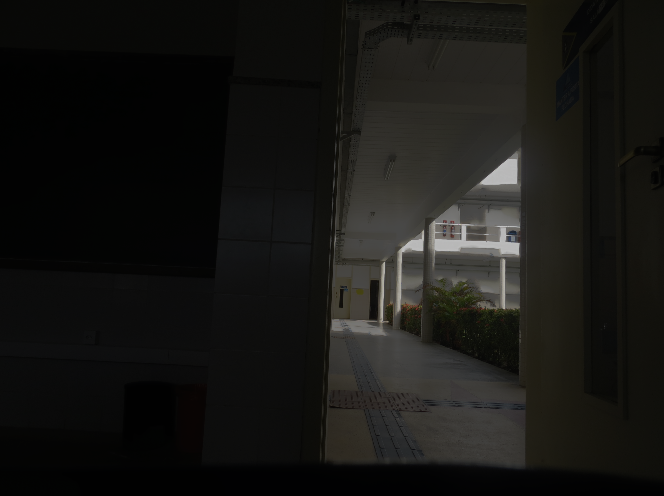
\includegraphics[height=6cm]{Sen/senSala-9,8EV}
    \label{figSenSalaA}
  }
  \quad %espaco separador
  \subfloat[Imagem visualizada com ganho de $-1,1$EV.]
  {
    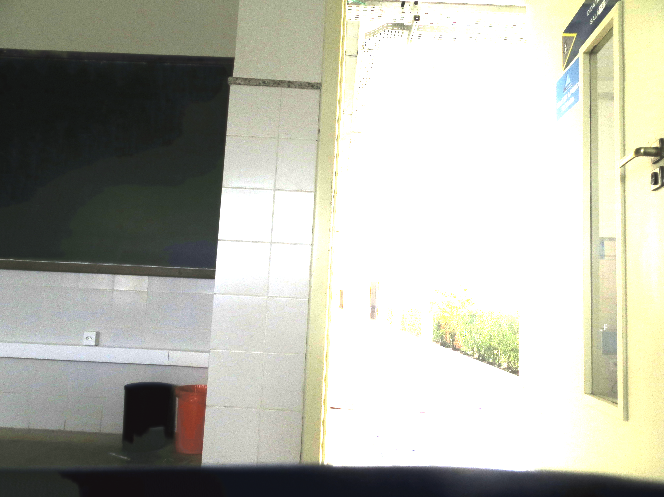
\includegraphics[height=6cm]{Sen/senSala-1,1EV}
    \label{figSenSalaB}
  }
  \caption{Imagem HDR gerada utilizando o método de Sen~\etal~\protect\cite{hdrMovimento}.}
  \label{figSenSala}
\end{figure}

\begin{figure}[H]
  \centering
  \subfloat[Imagem visualizada com ganho de $-1,3$EV.]
  {
    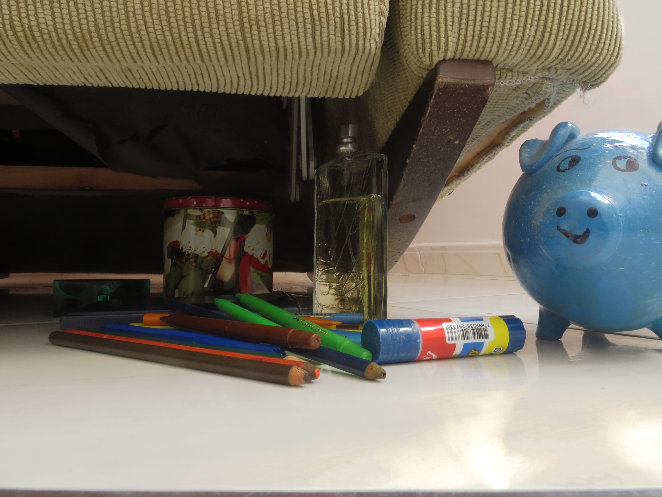
\includegraphics[height=6cm]{Sen/senPorquinho-1,3EV}
    \label{figSenPorquinhoA}
  }
  \quad %espaco separador
  \subfloat[Imagem visualizada com ganho de $2,5$EV.]
  {
    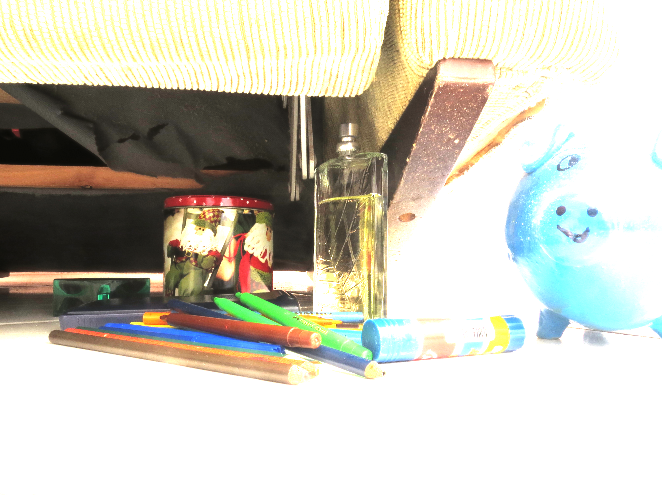
\includegraphics[height=6cm]{Sen/senPorquinho2,5EV}
    \label{figSenPorquinhoB}
  }
  \caption{Imagem HDR gerada utilizando o método de Sen~\etal~\protect\cite{hdrMovimento}.}
  \label{figSenPorquinho}
\end{figure}

\begin{figure}[H]
  \centering
  \subfloat[Imagem visualizada com ganho de $-0,6$EV.]
  {
    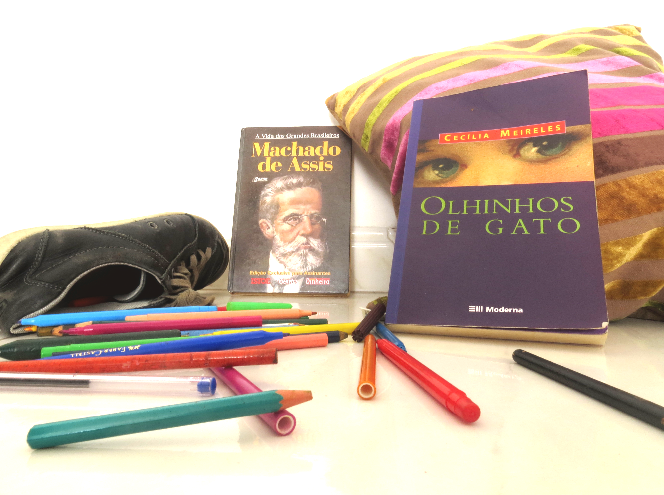
\includegraphics[height=6cm]{Sen/senOlhinhos-0,6EV}
    \label{figSenOlhinhosA}
  }
  \quad %espaco separador
  \subfloat[Imagem visualizada com ganho de $-3,4$EV.]
  {
    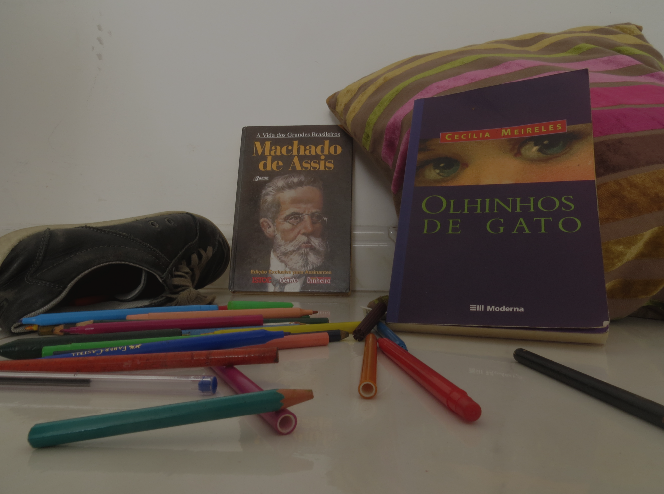
\includegraphics[height=6cm]{Sen/senOlhinhos-3,4EV}
    \label{figSenOlhinhosB}
  }
  \quad %espaco separador
  \subfloat[Imagem visualizada com ganho de $3,6$EV.]
  {
    
\includegraphics[height=6cm]{Sen/senOlhinhos3,6EV}
    \label{figSenOlhinhosC}
  }
  \caption{Imagem HDR gerada utilizando o método de Sen~\etal~\protect\cite{hdrMovimento}.}
  \label{figSenOlhinhos}
\end{figure}